%% LyX 2.2.3 created this file.  For more info, see http://www.lyx.org/.
%% Do not edit unless you really know what you are doing.
\documentclass[oneside,english]{extbook}
\usepackage[T1]{fontenc}
\usepackage[latin9]{inputenc}
\usepackage{geometry}
\geometry{verbose,tmargin=25mm,bmargin=25mm,lmargin=25mm,rmargin=25mm}
\setcounter{secnumdepth}{3}
\setcounter{tocdepth}{3}
\setlength{\parindent}{0bp}
\synctex=-1
\usepackage{babel}
\usepackage{float}
\usepackage{textcomp}
\usepackage{graphicx}
\usepackage{setspace}
\onehalfspacing
\usepackage[unicode=true,pdfusetitle,
 bookmarks=true,bookmarksnumbered=false,bookmarksopen=false,
 breaklinks=false,pdfborder={0 0 1},backref=false,colorlinks=false]
 {hyperref}

\makeatletter
%%%%%%%%%%%%%%%%%%%%%%%%%%%%%% User specified LaTeX commands.
\usepackage{amssymb}
\usepackage{color}
\usepackage{listings}
\definecolor{hellgelb}{rgb}{1,1,0.85}
\definecolor{colKeys}{rgb}{0,0,1}
\definecolor{colIdentifier}{rgb}{0,0,0}
\definecolor{colComments}{rgb}{1,0,0}
\definecolor{colString}{rgb}{0,0.5,0}
\lstset{
      language=Matlab,
      float=hbp,
      basicstyle=\footnotesize\ttfamily,
      identifierstyle=\color{colIdentifier},
      keywordstyle=\color{colKeys},
      stringstyle=\color{colString},
      commentstyle=\itshape\color{colComments},
      columns=fixed,
      tabsize=4,
      frame=single,
      framerule=1pt,
      extendedchars=true,
      showspaces=false,
      showstringspaces=false,
      numbers=left,
      numberstyle=\tiny\ttfamily,
      numbersep=1em,
      breaklines=true,
      breakindent=10pt,
      backgroundcolor=\color{hellgelb},
      breakautoindent=true,
      captionpos=t,
      xleftmargin=1em,
      xrightmargin=\fboxsep
}
\usepackage{lscape}
\usepackage{amsmath}
\usepackage{pifont}
\usepackage{color}
\usepackage{accents}
\delimitershortfall=-1pt
\let\Right\right
\let\Left\left
\makeatletter
\def\right#1{\Right#1\@ifnextchar){\!\right}{}}
\def\left#1{\Left#1\@ifnextchar({\!\left}{}}
\makeatother

\setcounter{MaxMatrixCols}{20}

\makeatother

\usepackage{listings}
\renewcommand{\lstlistingname}{Listing}

\begin{document}
\pagenumbering{gobble}

The robot's position is a big blue dot. Around the robot's position
is the position uncertainty ellipse, in blue, and finally, the$\pm\,\sigma_{\theta_t}$
of uncertainty in heading. At this position the robot sees 4 landmarks
relative to its own coordinate system. These landmarks are depicted
in green in the robot's coordinate system and they are also depicted
in green in the world coordinate system. So, these green dots are
simply the measurements transformed into the world coordinate system
according to the robot's current location and orientation. Remember,
the world's coordinate system is the robot's first coordinate system.
The estimated position for each landmark is depicted in magenta. These
positions are also part of our system state now, in addition to the
robot's estimated pose. The landmarks' position uncertainty ellipses
are also depicted in magenta.\\
\begin{figure}[H]
\centering{}\centering\includegraphics[scale=0.8]{../FIGURES/fig11}
\end{figure}

In the beginning the robot starts at an arbitrary position and orientation
in the world. At this moment, we have defined that the robot's uncertainty
in position and heading is zero. In the SLAM algorithm the built map
has its origin at the robot's initial position.\\
\begin{figure}[H]
\centering{}\centering\includegraphics[scale=0.8]{../FIGURES/fig12}
\end{figure}

The robot observes six cylinders from its initial pose. The discovered
landmarks' coordinates are added to the algorithm's state. Besides,
the position initial uncertainty of each discovered landmark is added
to the algorithm's covariance matrix. All this data is added to the
algorithm using the function\texttt{add\_landmark\_to\_state (initial\_coords)}.

\begin{align*}
\vec{\mu}_t\,=\,\begin{pmatrix}\mu_{x_t}\\\mu_{y_t}\\\mu_{\theta_t}\end{pmatrix} ~~\Longrightarrow ~~\vec{\mu}_t\,=\,\begin{pmatrix}\mu_{x_t}\\\mu_{y_t}\\\mu_{\theta_t}\\\mu_{{x_W}_1}\\\mu_{{y_W}_1}\\\vdots\\\mu_{{x_W}_N}\\\mu_{{y_W}_N}\end{pmatrix}
\end{align*}

\begin{gather*}
\Sigma_t\,=\,\begin{pmatrix}
\sigma_{x_t\hphantom{y_t}}^2 &\sigma_{x_ty_t} &\sigma_{x_t\theta_t}\\
\sigma_{x_ty_t} &\sigma_{y_t\hphantom{y_t}}^2 &\sigma_{y_t\theta_t}\\
\sigma_{x_t\theta_t} &\sigma_{y_t\theta_t} &\sigma_{\theta_t\hphantom{y_t}}^2
\end{pmatrix}\\\\
\Big\Downarrow\\\\
\Sigma_t\,=\,\begin{pmatrix}
\sigma_{x_t}^2 &\sigma_{x_ty_t} &\sigma_{x_t\theta_t} & 0 & 0 &\ldots & 0 & 0 &\ldots & 0 & 0\\
\sigma_{x_ty_t} &\sigma_{y_t}^2 &\sigma_{y_t\theta_t} & 0 & 0 &\ldots & 0 & 0 &\ldots & 0 & 0\\
\sigma_{x_t\theta_t} &\sigma_{y_t\theta_t} &\sigma_{\theta_t}^2 & 0 & 0 &\ldots & 0 & 0 &\ldots & 0 & 0\\
0 & 0 & 0 &\sigma_{{x_W}_0}^2 & 0 &\ldots & 0 & 0 &\ldots & 0 & 0\\
0 & 0 & 0 & 0 &\sigma_{{y_W}_0}^2 &\ldots & 0 & 0 &\ldots & 0 & 0\\
\vdots &\vdots &\vdots &\vdots &\vdots &\ddots &\vdots &\vdots &\vdots &\vdots &\vdots\\
0 & 0 & 0 & 0 & 0 &\ldots &\sigma_{{x_W}_j}^2 & 0 &\ldots & 0 & 0\\
0 & 0 & 0 & 0 & 0 &\ldots & 0 &\sigma_{{y_W}_j}^2 &\ldots & 0 & 0\\
\vdots &\vdots &\vdots &\vdots &\vdots &\vdots &\vdots &\vdots &\ddots &\vdots &\vdots\\
0 & 0 & 0 & 0 & 0 &\ldots & 0 & 0 &\ldots &\sigma_{{x_W}_N}^2 & 0\\
0 & 0 & 0 & 0 & 0 &\ldots & 0 & 0 &\ldots & 0 &\sigma_{{y_W}_N}^2
\end{pmatrix}
\end{gather*}

where $\sigma_{{x_W}_0}^2\,=\,\sigma_{{y_W}_0}^2\,=\,\ldots\,=\,\sigma_{{x_W}_N}^2\,=\,\sigma_{{y_W}_N}^2\,=\,\infty$
when these values are added to the algorithm's covariance matrix (for
practical purposes instead of $\infty$ we use 100 meters). These
initial uncertainty ellipses (in fact when $\sigma_{{x_W}_j}^2\,=\,\sigma_{{y_W}_j}^2$,
the major axis' length is equal the minor axis' length, so we have
a circle) are so big that we can't observe them in the GUI.

\newpage Main part of the algorithm:

\begin{lstlisting}
# Give values to algorithm's parameters
# Read data from files
for i in xrange(len(logfile.motor_ticks)): # Loop A
	# Prediction.
	control = array(logfile.motor_ticks[i]) * ticks_to_mm
	kf.predict(control)
    # Correction.
    observations = get_observations(logfile.scan_data[i], depth_jump, minimum_valid_distance, cylinder_offset, kf, max_cylinder_distance)
	for obs in observations: 			  # Loop B
		measurement, cylinder_world, cylinder_scanner, cylinder_index = obs
		if cylinder_index == -1:
			cylinder_index = kf.add_landmark_to_state(cylinder_world)
		kf.correct(measurement, cylinder_index)
	# Write data  to file
\end{lstlisting}

After the for loop labeled as B finishes its execution for the first
time the algorithm has obtained:

\begin{figure}[H]
\centering{}\centering\includegraphics[scale=0.8]{../FIGURES/fig13}
\end{figure}

From its initial pose the robot observes 6 landmarks. So the algorithm
adds the first landmark to the specific state and also to the covariance
matrix. Then the algorithm executes the correction stage using the
first landmark added previously. Then the algorithm adds the second
landmark to the specific state and also to the covariance matrix.
Then it executes the correction stage using two landmarks. Finally
when the algorithm has added the six landmarks and has executed 6
corrections stages (one per cylinder observation) the result is the
one shown in the previous figure.\\
The robot is stopped for a while in its initial pose. So, the prediction
stage doesn't modify the algorithm's specific state. From this pose
the robot observes 6 cylinders in several scans. Each one of those
scans with 6 cylinders implies the execution of the for loop labeled
as B with 6 iterations (one iteration per observed cylinder), therefore,
6 correction stages. In this occasion, all the cylinders observed
are already present in the algorithm's specific state. So, after the
last correction stage, for the last cylinder observed in the last
scan taken from the same robot's pose, the algorithm has reduced the
landmarks' uncertainty ellipses considerably, as it is show below.\\
\begin{figure}[H]
\centering{}\centering\includegraphics[scale=0.8]{../FIGURES/fig14}
\end{figure}

If the robot moves then its pose uncertainty (position uncertainty
and heading uncertainty) starts to get larger and larger, and as usual,
it is especially large when the robot turns left for the first time
because it doesn't observe many landmarks at that point.

\begin{figure}[H]
\centering{}\centering\includegraphics[scale=0.8]{../FIGURES/fig15}
\end{figure}

\begin{figure}[H]
\centering{}\centering\includegraphics[scale=0.8]{../FIGURES/fig16}
\end{figure}

If the robot goes on its uncertainty pose gets smaller again.

\begin{figure}[H]
\centering{}\centering\includegraphics[scale=0.8]{../FIGURES/fig17}
\end{figure}

Now let's look at the landmarks' uncertainties. The error ellipse
for the landmarks A and E is small but the error ellipse for the landmarks
B, C and F is larger. The reason for this is that our coordinate system
is actually anchored to the point O. This point has 0 variance in
position and orientation and the further away a cylinder is from the
robot the first time it is observed the larger the error will be,
and even though the robot drives around for a while these uncertainties
will stay the same.

\begin{figure}[H]
\centering{}\centering\includegraphics[scale=0.8]{../FIGURES/fig18}
\end{figure}

Now, let's look at landmark D. In the beginning, while the robot is
stopped in its initial pose, the robot observes the landmark D for
a while, so the uncertainty ellipse of this landmark gets smaller,
relatively fast.

\begin{figure}[H]
\centering{}\centering\includegraphics[scale=0.8]{../FIGURES/fig20}
\end{figure}

\begin{figure}[H]
\centering{}\centering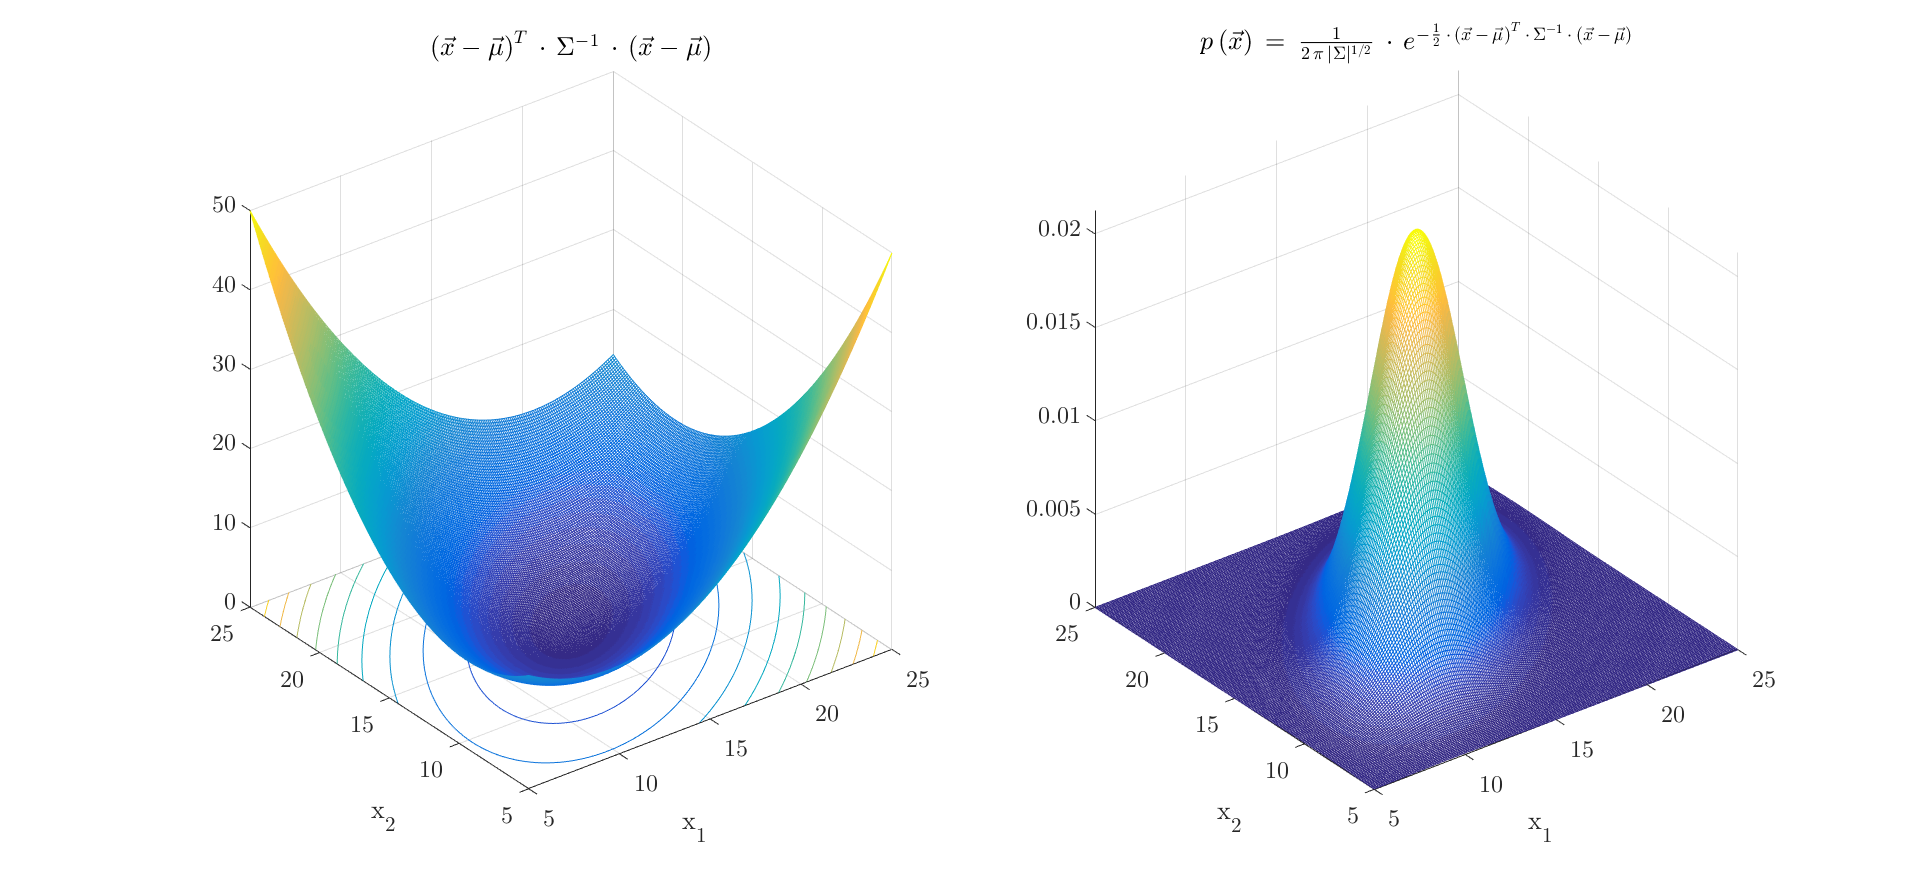
\includegraphics[scale=0.8]{../FIGURES/fig21}
\end{figure}

\begin{figure}[H]
\centering{}\centering\includegraphics[scale=0.8]{../FIGURES/fig22}
\end{figure}

Now, as the robot moves, it still observes the landmark D, but the
uncertainty ellipse of that landmark doesn't get smaller as fast as
it did previously because now the robot's pose has also accumulated
some uncertainty.

\begin{figure}[H]
\centering{}\centering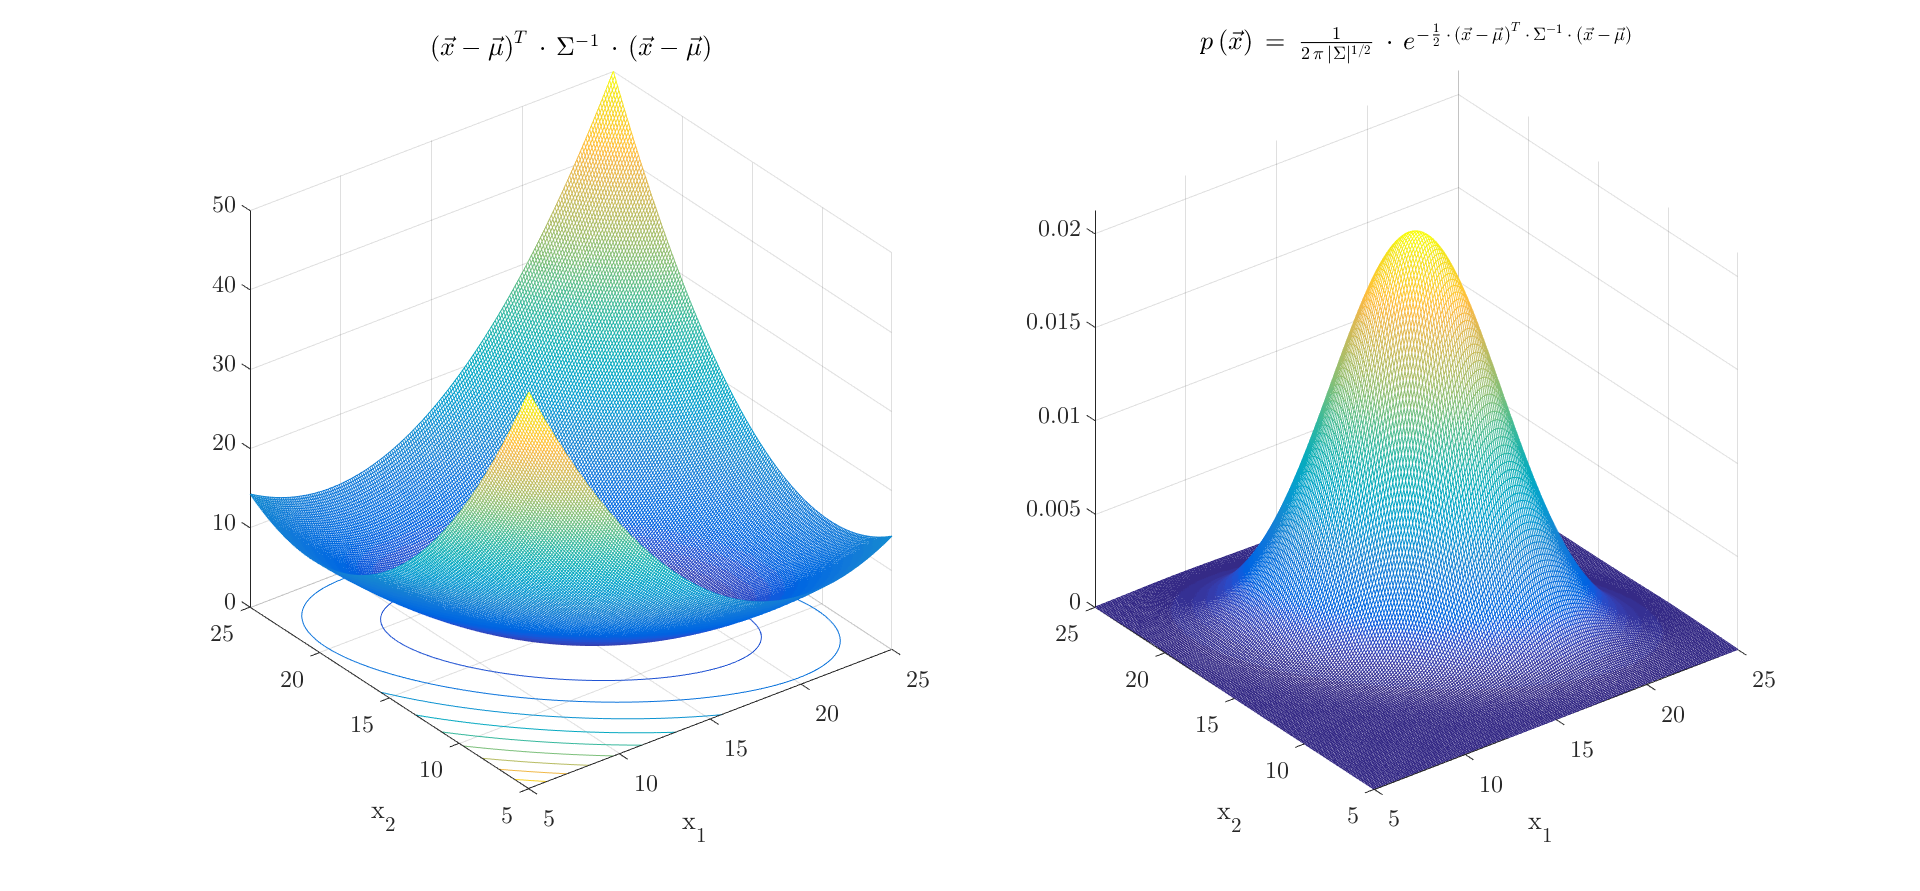
\includegraphics[scale=0.8]{../FIGURES/fig23}
\end{figure}

\begin{figure}[H]
\centering{}\centering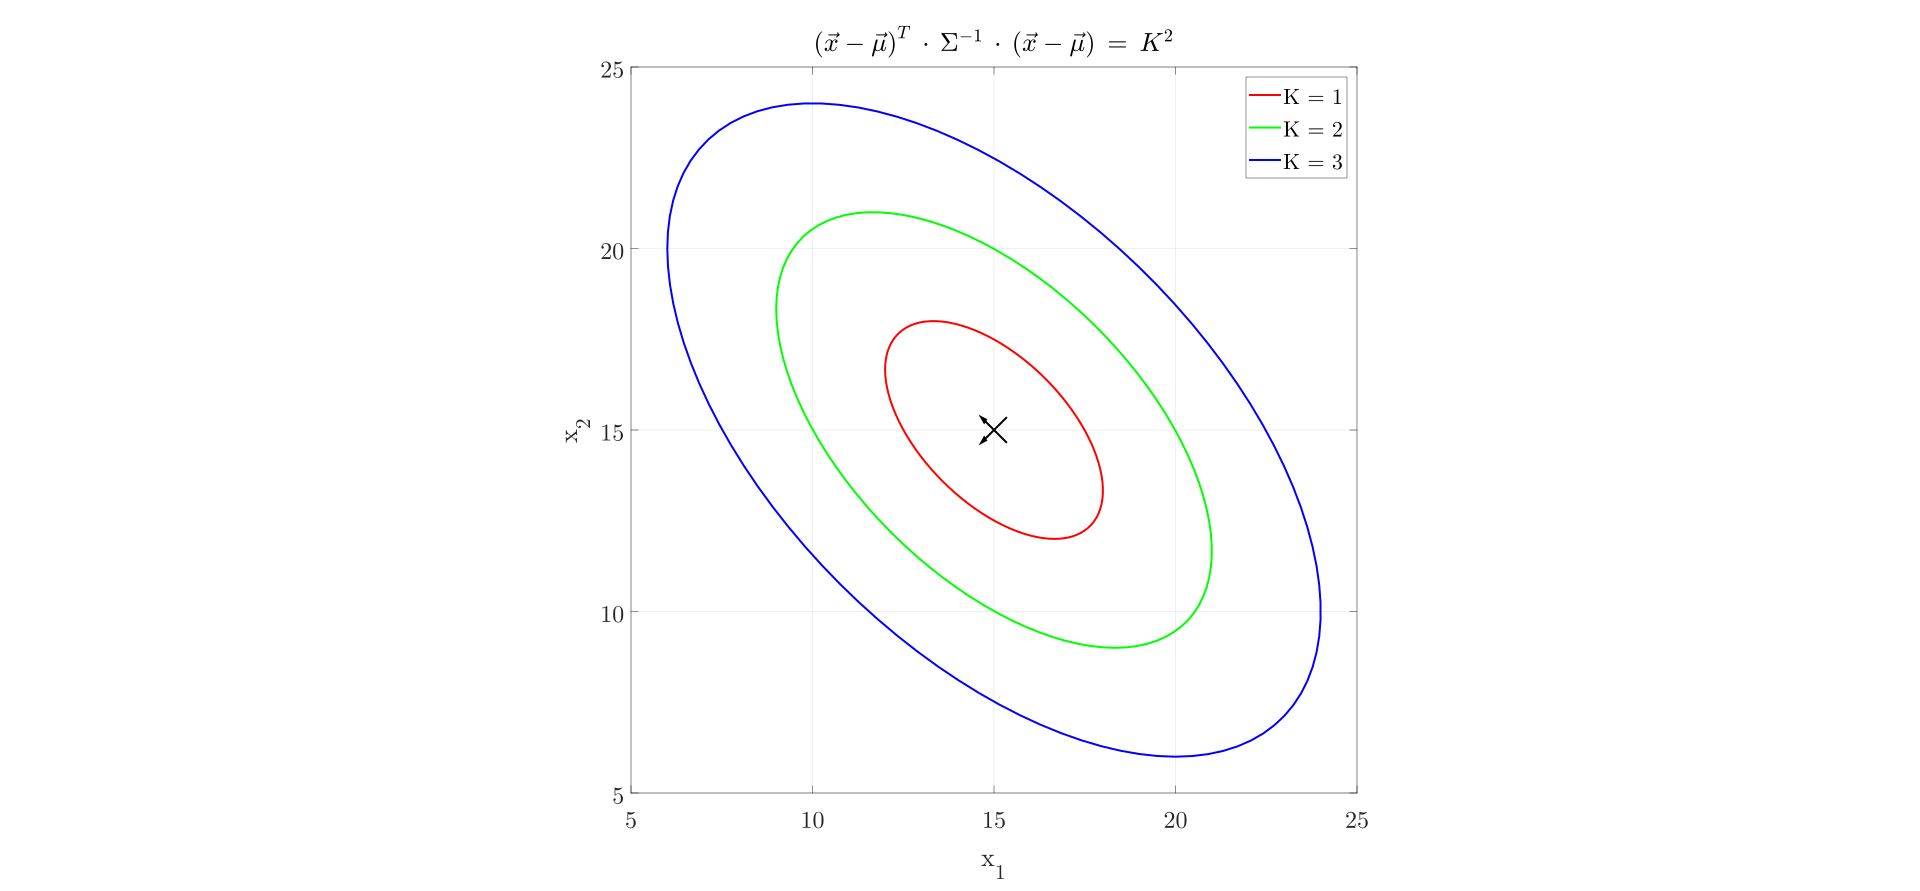
\includegraphics[scale=0.8]{../FIGURES/fig24}
\end{figure}

As long as the robot has an observation that is tied to a landmark
(the green point close to each landmark) the uncertainty ellipse of
that landmark gets smaller. When the robot doesn't have an observation
of a landmark anymore the size of the uncertainty ellipse for that
landmark stays the same but that landmark's position will move a little
bit when the landmarks in the vicinity move. But again, the size of
the uncertainty ellipse of the non-observed landmarks will stay the
same.

\begin{figure}[H]
\centering{}\centering\includegraphics[scale=0.8]{../FIGURES/fig25}
\end{figure}

Now, the robot starts observing the landmark D again, and its uncertainty
ellipse gets smaller again.

\begin{figure}[H]
\centering{}\centering\includegraphics[scale=0.8]{../FIGURES/fig26}
\end{figure}

Now, the landmark D is out of the robot's field of view again and
the uncertainty ellipse of this landmark stays the same.

\begin{figure}[H]
\centering{}\centering\includegraphics[scale=0.8]{../FIGURES/fig27}
\end{figure}

Now, the robot starts observing the landmark D again, and its uncertainty
ellipse gets smaller again.

\begin{figure}[H]
\centering{}\centering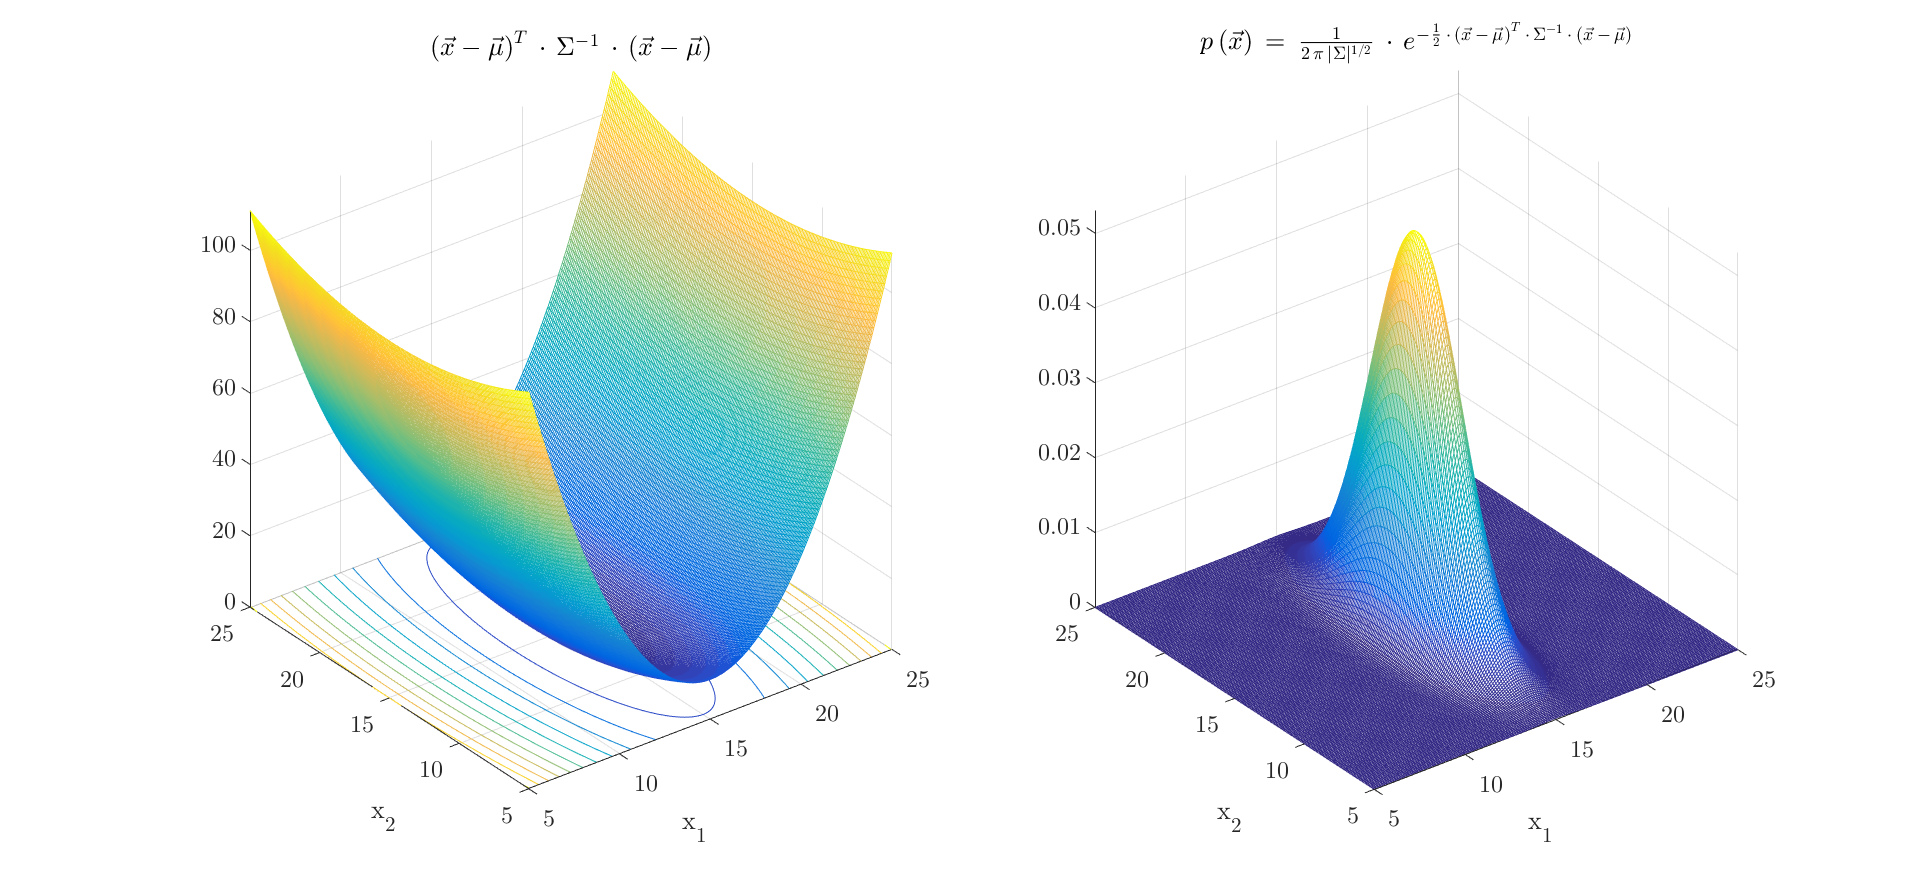
\includegraphics[scale=0.8]{../FIGURES/fig28}
\end{figure}

Therefore, basically, whenever the robot has a landmark observation,
i.e, whenever there is a green point tied to a landmark in the GUI,
the algorithm adds information and when the information increases
the uncertainty decreases.

Now let's change the covariance matrix:

\begin{gather*}
\Sigma_t\,=\,\begin{pmatrix}
\sigma_{x_t\hphantom{y_t}}^2\,=\, 0 &\sigma_{x_ty_t}\,=\, 0 &\sigma_{x_t\theta_t}\,=\, 0\\
\sigma_{x_ty_t}\,=\, 0 &\sigma_{y_t\hphantom{y_t}}^2\,=\, 0 &\sigma_{y_t\theta_t}\,=\, 0\\
\sigma_{x_t\theta_t}\,=\, 0 &\sigma_{y_t\theta_t}\,=\, 0 &\sigma_{\theta_t\hphantom{y_t}}^2\,=\, 0
\end{pmatrix}\\\\
\Big\Downarrow\\\\
\Sigma_t\,=\,\begin{pmatrix}
\sigma_{x_t\hphantom{y_t}}^2\,=\, 10 &\sigma_{x_ty_t}\,=\, 0\hphantom{0} &\sigma_{x_t\theta_t}\,=\, 0\hphantom{\left.\dfrac{00}{000}\,\pi\right)^2}\\
\sigma_{x_ty_t}\,=\, 0\hphantom{0} &\sigma_{y_t\hphantom{y_t}}^2\,=\, 10 &\sigma_{y_t\theta_t}\,=\, 0\hphantom{\left.\dfrac{00}{000}\,\pi\right)^2}\\
\sigma_{x_t\theta_t}\,=\, 0\hphantom{0} &\sigma_{y_t\theta_t}\,=\, 0\hphantom{0} &\sigma_{\theta_t\hphantom{y_t}}^2\,=\,\left(\dfrac{10}{180}\,\pi\right)^2
\end{pmatrix}
\end{gather*}
\begin{center}
\begin{figure}[h]
\centering{}\centering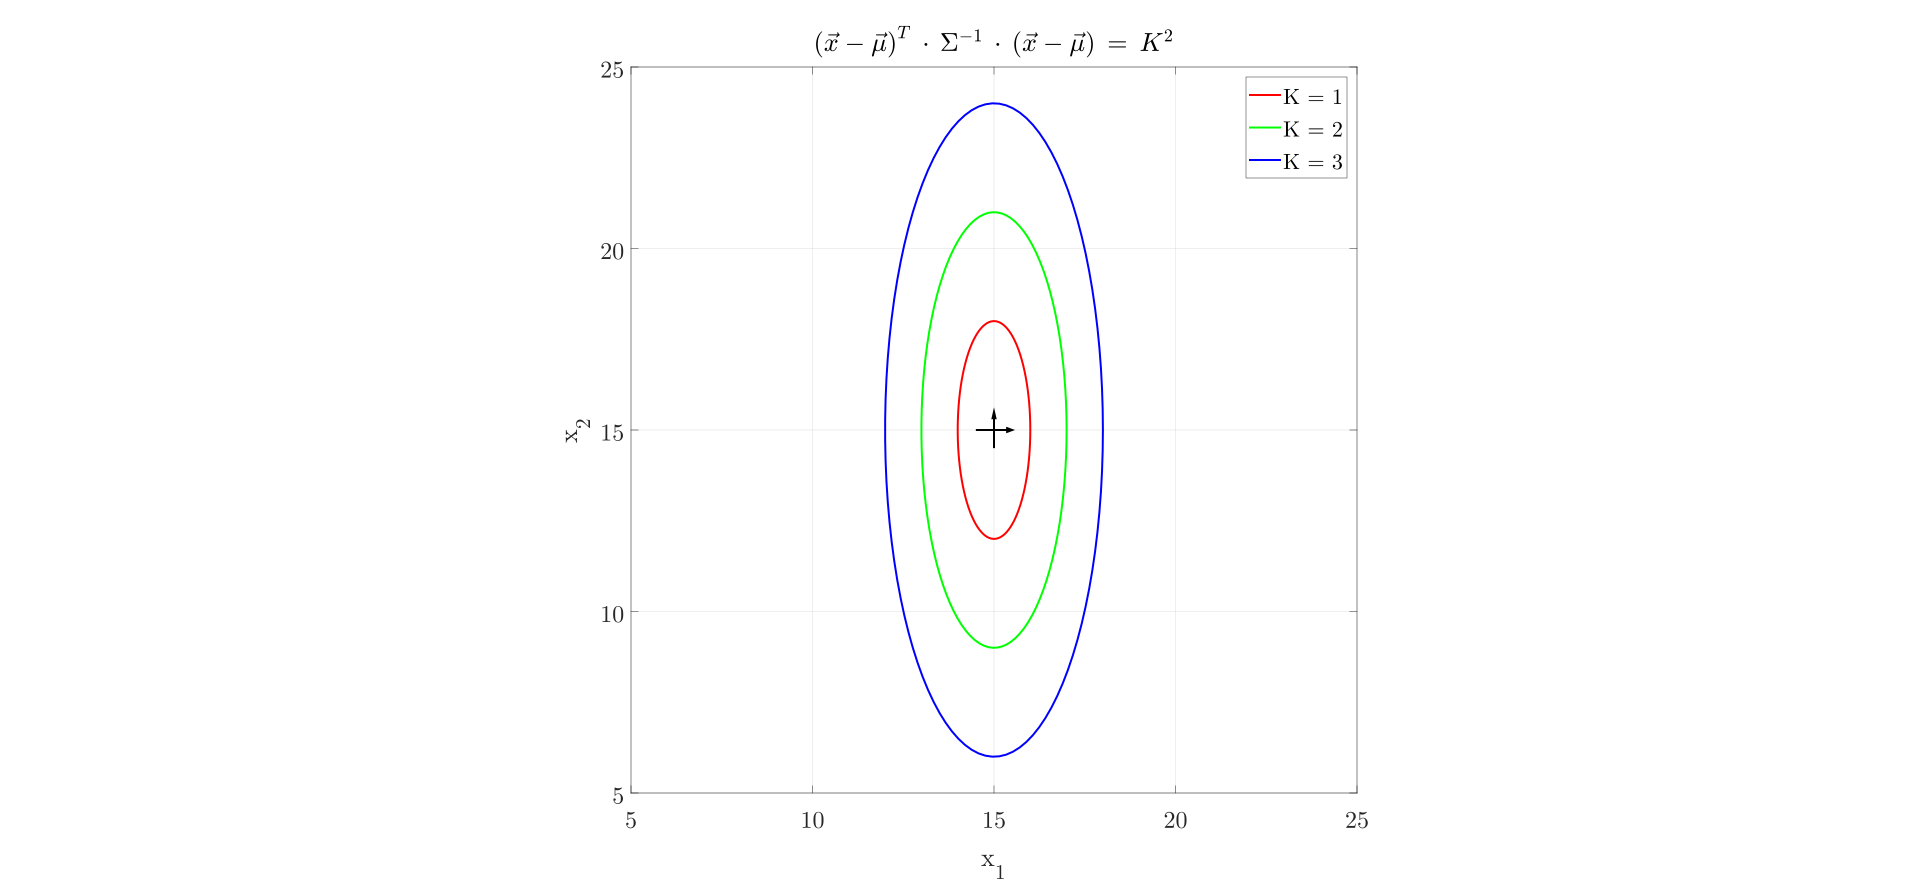
\includegraphics{../FIGURES/fig29}
\end{figure}
\par\end{center}

After the robot drives for a while we\textasciiacute ll see the size
of the uncertainty ellipse of each landmark doesn't get smaller anymore.
\begin{center}
\begin{figure}[H]
\centering{}\centering\includegraphics[scale=0.8]{../FIGURES/fig31}
\end{figure}
\par\end{center}

\begin{center}
\begin{figure}[H]
\centering{}\centering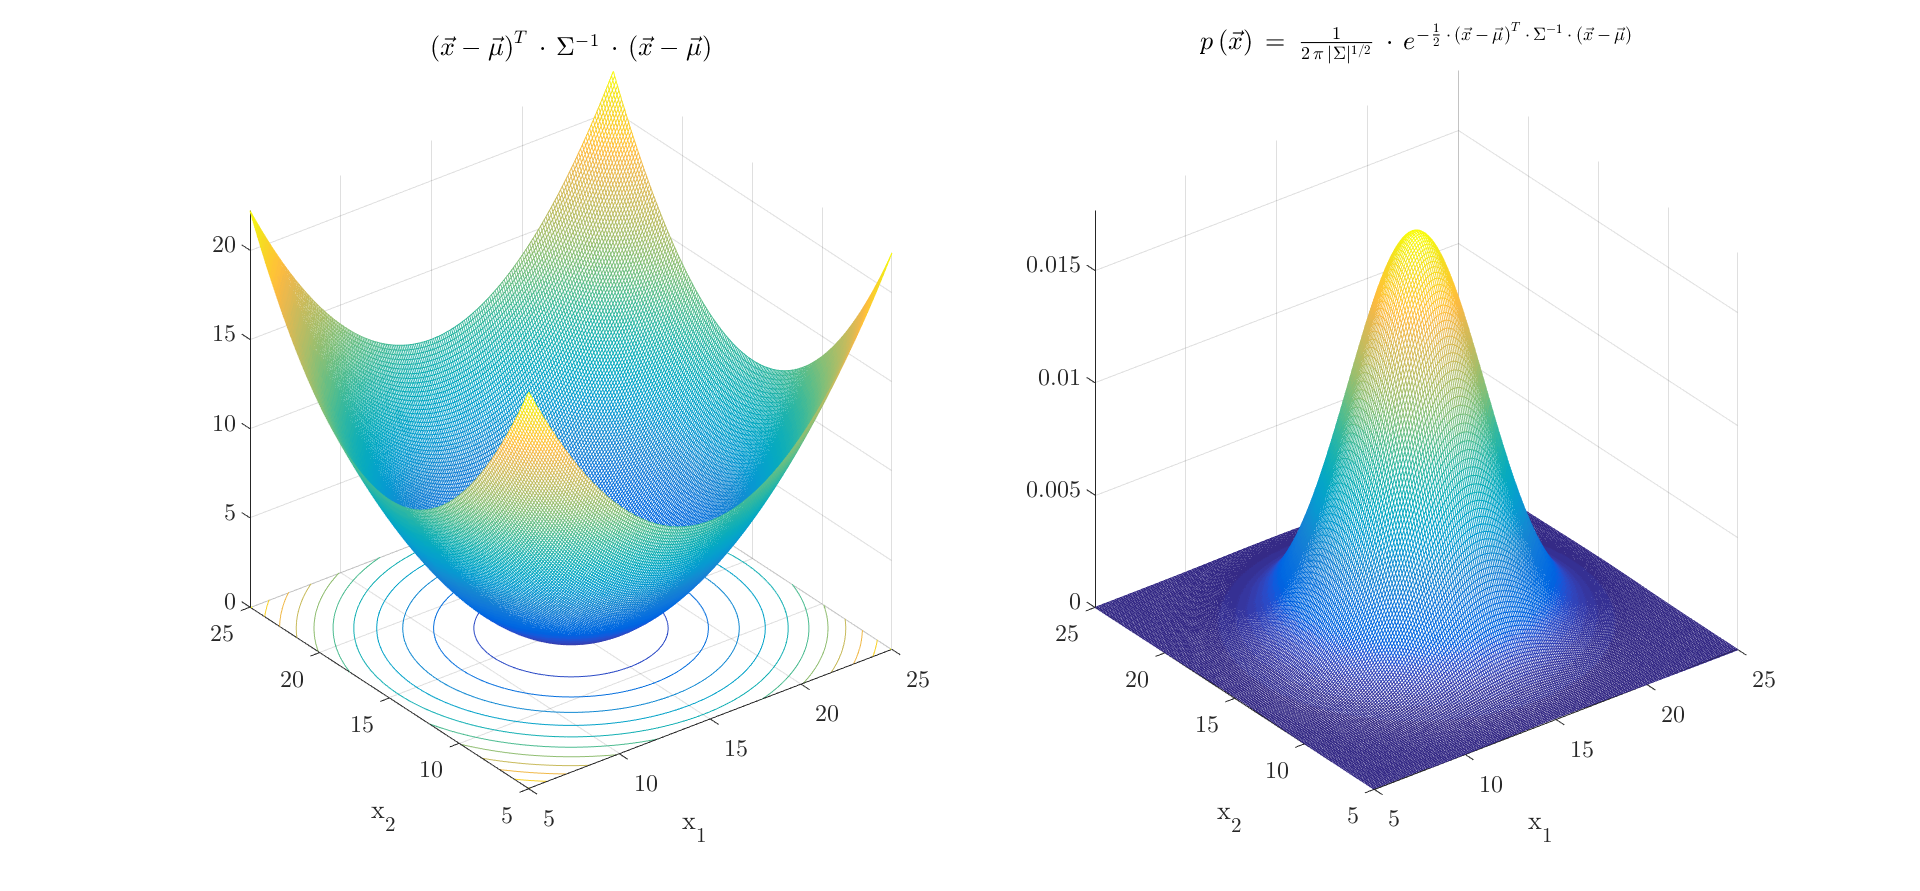
\includegraphics[scale=0.8]{../FIGURES/fig32}
\end{figure}
\par\end{center}

\begin{center}
\begin{figure}[H]
\centering{}\centering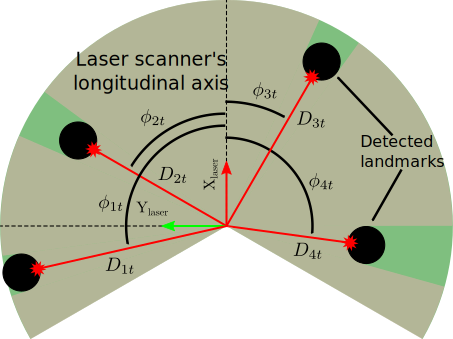
\includegraphics[scale=0.8]{../FIGURES/fig33}
\end{figure}
\par\end{center}

\begin{center}
\begin{figure}[H]
\centering{}\centering\includegraphics[scale=0.8]{../FIGURES/fig34}
\end{figure}
\par\end{center}

In the end, the size of the landmarks' uncertainty ellipses, the size
of the position uncertainty ellipse for the robot and the size of
the heading uncertainty sector for the robot are larger than in the
previous case. Why is this the case? Simply because the overall uncertainty
is tied to the robot's uncertainty in the initial pose, i.e, the pose
at the point labeled as O. Therefore, if you have a large variance
in the beginning the algorithm never be able to obtain small variances
for the landmarks' positions, no matter how many relative measurements
the robot obtains. So, the uncertainty ellipses for the landmarks
won't get smaller and since the robot uses the landmarks in the correction
step of the EKF, the uncertainty for the robot won't get smaller either.\\

If we make the variances even larger:

\begin{gather*}
\Sigma_t\,=\,\begin{pmatrix}
\sigma_{x_t\hphantom{y_t}}^2\,=\, 30 &\sigma_{x_ty_t}\,=\, 0\hphantom{0} &\sigma_{x_t\theta_t}\,=\, 0\hphantom{\left.\dfrac{00}{000}\,\pi\right)^2}\\
\sigma_{x_ty_t}\,=\, 0\hphantom{0} &\sigma_{y_t\hphantom{y_t}}^2\,=\, 30 &\sigma_{y_t\theta_t}\,=\, 0\hphantom{\left.\dfrac{00}{000}\,\pi\right)^2}\\
\sigma_{x_t\theta_t}\,=\, 0\hphantom{0} &\sigma_{y_t\theta_t}\,=\, 0\hphantom{0} &\sigma_{\theta_t\hphantom{y_t}}^2\,=\,\left(\dfrac{20}{180}\,\pi\right)^2
\end{pmatrix}
\end{gather*}

we will easily see the effect.

\begin{center}\begin{figure}[H]\centering{}\includegraphics[scale=1.0]{../FIGURES/fig36.png}\end{figure}\par\end{center}

So, the robot starts now with a larger associated uncertainty and
as it moves the larger variances in the initial pose translates to
a larger variance of the landmarks' positions, of the robot's position
and of the robot's heading, no matter how many measurements the algorithm
integrates during the trip.

\begin{center}\begin{figure}[H]\centering{}\includegraphics[scale=0.8]{../FIGURES/fig37.png}\end{figure}\par\end{center}
\begin{center}\begin{figure}[H]\centering{}\includegraphics[scale=0.8]{../FIGURES/fig38.png}\end{figure}\par\end{center}
\begin{center}\begin{figure}[H]\centering{}\includegraphics[scale=0.8]{../FIGURES/fig39.png}\end{figure}\par\end{center}
\begin{center}\begin{figure}[H]\centering{}\includegraphics[scale=0.8]{../FIGURES/fig40.png}\end{figure}\par\end{center}

Finally let's have a look at the maximum cylinder distance. This distance
is set, by default, to 50 cm. Now let's set this distance to 40 cm.
Initially the algorithm gets exactly the same results as previously.
But after a while, the robot has the wrong heading and so the cylinder
that it observes is considerably far away from the landmark that should
be associated to it. Anyway, the cylinder is close enough to the proper
landmark according to the 40 cm threshold, so the cylinder is assigned
to the correct landmark.

But in the next step the observed cylinder is too far away from any
of the landmarks, therefore, the algorithm sets up a new landmark
with position variances set to infinity.

\begin{center}\begin{figure}[H]\centering{}\includegraphics[scale=0.8]{../FIGURES/fig42.png}\end{figure}\par\end{center}

The robot observes more landmarks again, so it corrects the landmarks'
positions and what we see is that after a while the newly inserted
landmark is moved very close to the old landmark. What we see is that
the landmark assignment is pretty simple and it is also brittle.

\begin{center}\begin{figure}[H]\centering{}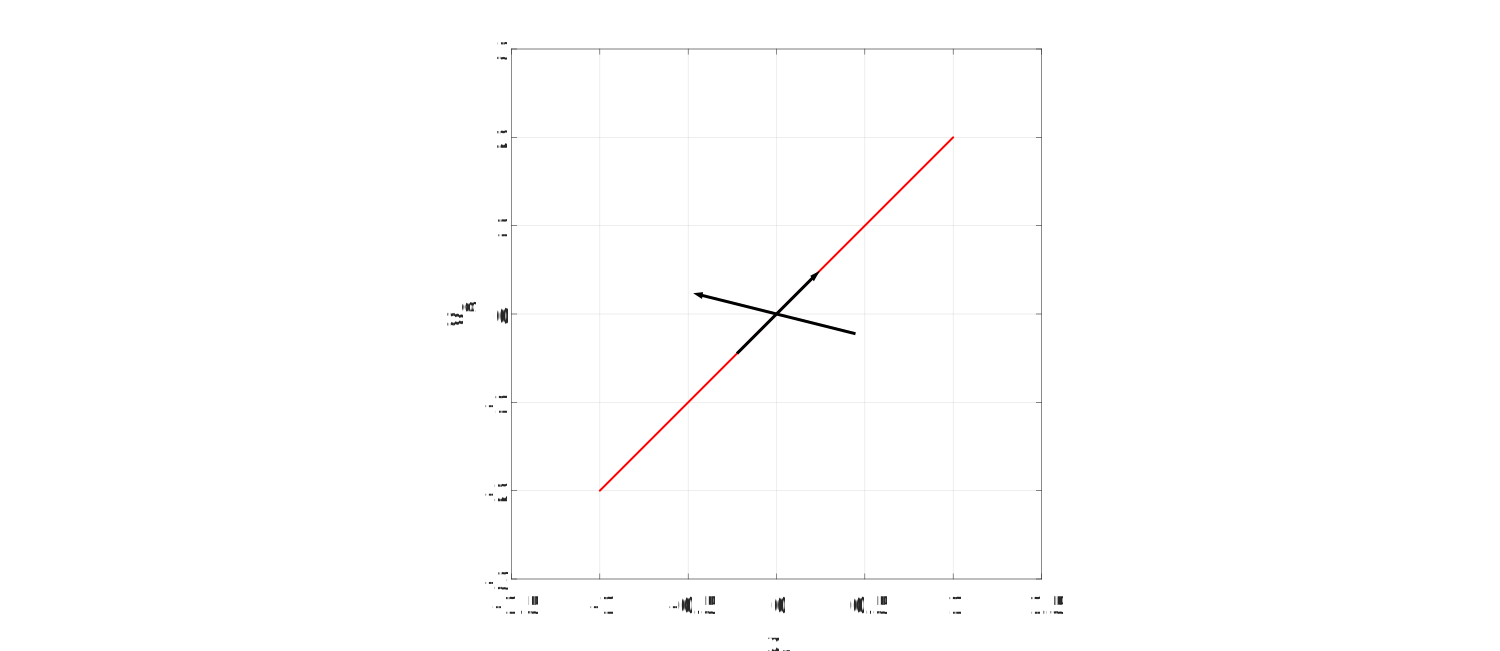
\includegraphics[scale=0.8]{../FIGURES/fig43.png}\end{figure}\par\end{center}
\begin{center}\begin{figure}[H]\centering{}\includegraphics[scale=0.8]{../FIGURES/fig44.png}\end{figure}\par\end{center}
\begin{center}\begin{figure}[H]\centering{}\includegraphics[scale=1.0]{../FIGURES/fig45.png}\end{figure}\par\end{center}

Let's make the maximum cylinder distance even smaller: 30 cm.

The algorithm starts perfectly, as in the previous case. When the
robot moves around the first corner the algorithm makes new landmark
and a bit more later it creates one more landmark. In the end the
algorithm obtains ten landmarks instead of six. This behavior shows
us how brittle this landmark assignment process actually is and obviously
you could try to improve the algorithm. For example, we could think
about unifying landmarks which turn out to be close after observing
them for a while but there is other techniques.

\begin{center}\begin{figure}[H]\centering{}\includegraphics[scale=0.8]{../FIGURES/fig46.png}\end{figure}\par\end{center}
\begin{center}\begin{figure}[H]\centering{}\includegraphics[scale=0.8]{../FIGURES/fig47.png}\end{figure}\par\end{center}
\begin{center}\begin{figure}[H]\centering{}\includegraphics[scale=0.8]{../FIGURES/fig48.png}\end{figure}\par\end{center}
\begin{center}\begin{figure}[H]\centering{}\includegraphics[scale=0.8]{../FIGURES/fig49.png}\end{figure}\par\end{center}
\end{document}
